%\documentclass{tise_style}
%\usepackage{natbib}
%Having trouble getting tise_style to compile correctly in RStudio, will re-run it with this before submission

%-----------------------------------------------------------------------------------------------------
%Substitute this all with tise_style
\documentclass[12pt]{article}
\usepackage{natbib}  % used for citations
\usepackage[parfill]{parskip} %used for formatting style of text
\usepackage{url}
\usepackage{graphicx}
% Sets margins to 1 in
%\addtolength{\oddsidemargin}{-.5in}%
%\addtolength{\evensidemargin}{-.5in}%
%\addtolength{\textwidth}{1in}%
%\addtolength{\textheight}{1.3in}%
%\addtolength{\topmargin}{-.8in}%
%-----------------------------------------------------------------------------------------------------



\title{Enter our title here}

\author{Tessa Mcdonnel, Shannon Pileggi,  \\Statistics Department, California Polytechnic State University, San Luis Obispo}
%\author{Shannon Pileggi \\Statistics Department, California Polytechnic State University, San Luis Obispo}




\begin{document}


\maketitle

\section{Introduction}

Questions: 

1) should i add more about how it can be used in a flipped classroom?

2) how to get side by side pictures (for the teach editor code vs. preview)?

3) also, what is the best way to add pictures? They are not inserted in the pdf where i have the code

4) what are the bottom comments about the citations?

5) should i add that the courses are written in Hadley Wickham style?

It is no suprise that technology plays a vital role in practicing statistics and as the technological revolution continues to
unfold, the use of statistical software has become increasingly emphasized in education (**do i need to cite this**). By integrating the
capabilities of technology in introductory statistics courses, students can explore fundamental concepts by analyzing and
interpreting real data sets \cite{Chance2007, Hardin2015, Horton2014}, giving them an authentic view of how statistics is practiced outside of the
classroom \cite{Wang2017}. The revised 2016 \textit{Guidelines for Assessment and Instruction in Statistics Education}
(GAISE) College Report has also prompted the use of more technology in introductory statistics courses, encouraging educators
to use technology "as a way to explore conceptual ideas and enhance student learning" \cite{AmericanStatisticalAssociation2016}.

The goal for any introductory statistics course is to help students develope the ability to think statistically
\cite{AmericanStatisticalAssociation2016}.
Introducing technology into the curriculum can greatly strengthen this ability by illustrating statistical concepts such as
variability, randomness and hypothesis testing. Although numerous statistical technologies exist, \textit{R} and \textit{R Studio}
provide extensive statistical capabilites (free of charge) and are commonly used in statistics courses \cite{Chance2007}. R
allows students to explore real-world data sets which can not only enhance their understanding of concepts, but can also spark
an interest in the domain of statistics \cite{Wang2017}.

With this increased use of R in classrooms, there is a need for an effective way to get students familiar with statistical software
\cite{Baumer2014}. While Rsoftware provides users with extraordinary abilities there is no doubt a steep learning curve. To facilitate
this transition to R programming, popular interactive teaching technologies have been created including Swirl (need to cite this?), LearnR
and TryR. 
These tools allow students to work through coding problems while recieving immediate feedback in and out of the classroom. Swirl is an
open source R software package that allows students to learn R programing in their R console. This interactive learning tool
contains several pre-existing lessons but what makes Swirl so popular is its versitality; educators can create their own
lesson (or tailor a pre-existing one) to fit their curriculum and assign it to students \cite{Carchedi2014}.
While swirl can be linked to a Massive Open Online Courses (MOOCs) like Coursera through API, integration of learning management 
systems (LMS) is not available for the classroom.

*I'm confused about LearnR and think someone else should write about it.*

TryR (Code School 2014) is a web-based programs and does not have this reproducible capability. Since public content authoring
is not available, educators are limited on what they can teach their students. The R console can be intimidating to
introductory statistics students so an advantage of a web-based teaching tool is
the clean and easy to use interface. This is an important quality given that a lot of the time students struggle more with
software than the statistical concepts themselves \cite{Hare2017}. When students only need their web browser to participate,
all installation complications are avoided and valuable class time can be focused on the statistics, not computer issues.

DataCamp has the same reproducable capabilities as Swirl but is a web-based application; educators can
create their own courses that coincide with their lessons and students can access the course without having to install R.
Courses are available through the DataCamp website and students can access the lesson through their web-browser on a laptop,
tablet or moble device, making the courses accessable to anyone with an internet connection. 
The DataCamp website offers pre-existing free community courses as well as specialized 'Premium' classes that you need to purchase. 
However, when used for academic purposes the premium DataCamp content is also free of charge.. (i'll come back to this).
Any college educator can create a classroom group on the DataCamp website, add student's to the group, assign pre-existing 
'community' courses or assign a course that they've created for the particular class. 

The collection of community courses avaiable at DataCamp inlcude a wide range of topics from 'Introduction to R' to
'Quantitative Risk Management in R' so novice through advanced programming students will benefit.
DataCamp can be used in the classroom in a number of ways: as traditional homework assignments, as an
activity during lab periods, as pre-class assignments for a flipped classroom, and even as a test or assessment tool.

A feature that sets DataCamp apart from competing technologies is the ability to track student progress. Educators
can set deadlines for assignments and easily see not only when students complete an assignment but also which sections the
students had trouble with in a detailed report (datacamp/teach website). Student scores can be automatically updated to a
current gradebook when you link the schools' learning management system (LMS) to DataCamp, allowing for a smooth integration of student work.

Each chapter in a DataCamp course is made up of modular exercises. Modulariy is critical component in designing a statistical
learning tool because it allows independent pieces to be easily added, modified or removed from the entire functionality
\cite{Hare2017}. Course exercises can be added, modified, or deleted as new topics arise and instructors can tailor
these exercises to meet the needs of a particular class. The only disadvantage of the modularity feature is that the sessions
are not cummulative; every exercise begins with a clear workspace so an object defined in a previous exercise needs to be
defined again. Each of these exercises can be given a number of redeemable points which the students can see when they begin
the exercise, introducing a gamification feature to the learning experience. If the student completes the exercise without
any help they will recieve the full points. If they ask for a hint, 30 percent of the available points will be deducted and
all of the points will be deducted if they ask for the entire answer. When in a classroom group, students can view their
progress (points and chapters completed) as well as then progress of their peers. This can help students perform better
because they want to be on par with the rest of the class; furthermore, when students can see the number of available points
for an exercise it will motivate them to meet their personal achievement goals. \citep{Chang2016}.


\section{How to Use DataCamp}

\subsection{Pre-existing R courses}
DataCamp has a range of available free community courses that educators can utilize for supplimental R practice.

\subsection{Creating a DataCamp Course}
To build a course on DataCamp you will first need to create a DataCamp account by visiting \url{www.datacamp.com/teach} and
a GitHub account \url{https://github.com}. The simplest way to begin building the course is to use the templete course files from the 'Create
DataCamp Course' dialog. This will automatically create a GitHub repository that is linked to DataCamp; any changes that are
make through DataCamp will update the GitHub repository and visa versa. Every DataCamp course is linked through GitHub version control,
allowing statistics educators to easily collaborate and reproduce code. To add collaborators to the course, go to the course repository
on GitHub and under 'Settings' you can select the 'Collabroators' tab and enter the usernames of people you want to collaborate with.



The GitHub repository will contain three files: README.md, course.yml, and chapter1.Rmd.
Readme.md contains helpful information of how to get started, citing resourses to learn more about the process.
course.yml is a file that contains general information about the course you're creating: title, university, description,
difficulty level, ect.
chapter1.Rmd is a template chapter file with examples of 'normal' interative coding exercises and multiple choice questions.
To add more chapters to an R course, create new files in the repository and name them chapter1.Rmd, chapter2.Rmd, chapter3.Rmd
ect.

When starting to create a DataCamp course, it is helpful to view code from pre-existing community courses which can be found on GitHub.
You can use these files as a guide to build your own course or duplicate the repository and tailor the content to fit specific needs.
The DataCamp github repository contains links to the code for available courses; one of the most helpful when starting to build a course 
is 'datacamp/courses-intro-r' which contains the source files for the 'Intoduction to R' course.

Educators are able to edit their courses in a number of ways but the 'Teach Editor' located in the teach dashboard is the
most straight forward editor. The 'Teach Editor' is specifically designed to make the creation process of a DataCamp course
as painless as possible, allowing writers to edit, preview, save changes and synchronize to a GitHub repository. Editing can
also be done through GitHub's online editor and through git locally but these methods do not allow for automatic content
viewing.



DataCamp courses may contain 3 different types of exercises: Normal, Multiple choice, and video.

A 'NormalExercise' is an interactive coding exercise containing a lesson section, instructions, pre-exercise code, sample
code, hint, solution and a submission correctness testing coded (SCT). However, the interface for students (or the 'Preview
mode) only includes the lesson, Instructions, R script panel and a R console panel.



\begin{figure}[h]
  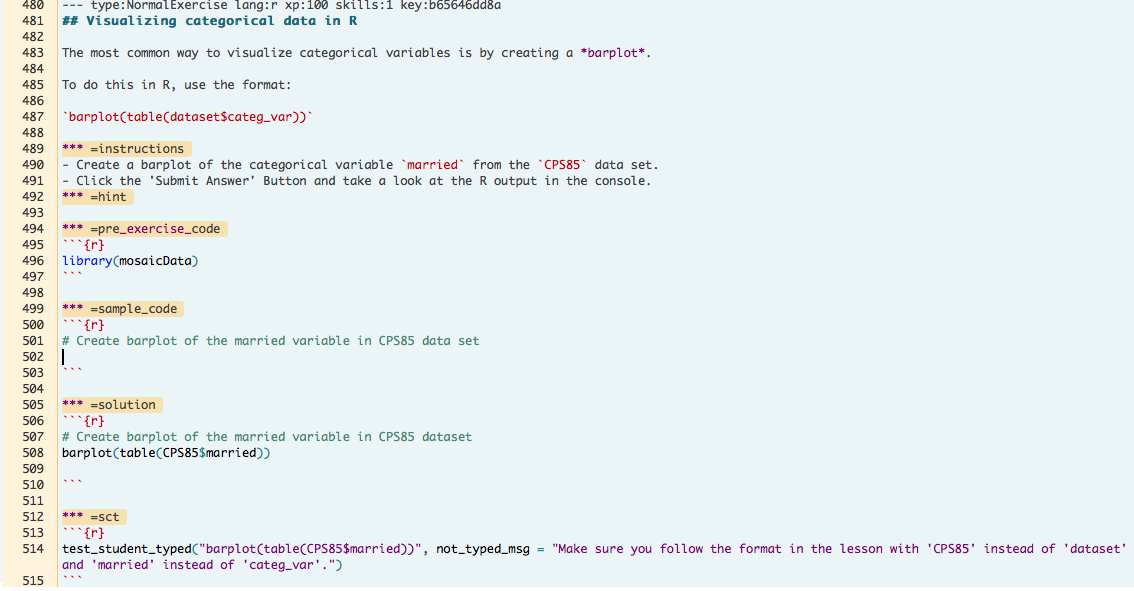
\includegraphics[scale = 0.2] {edit.jpg}
\end{figure}


\begin{figure}[h]
  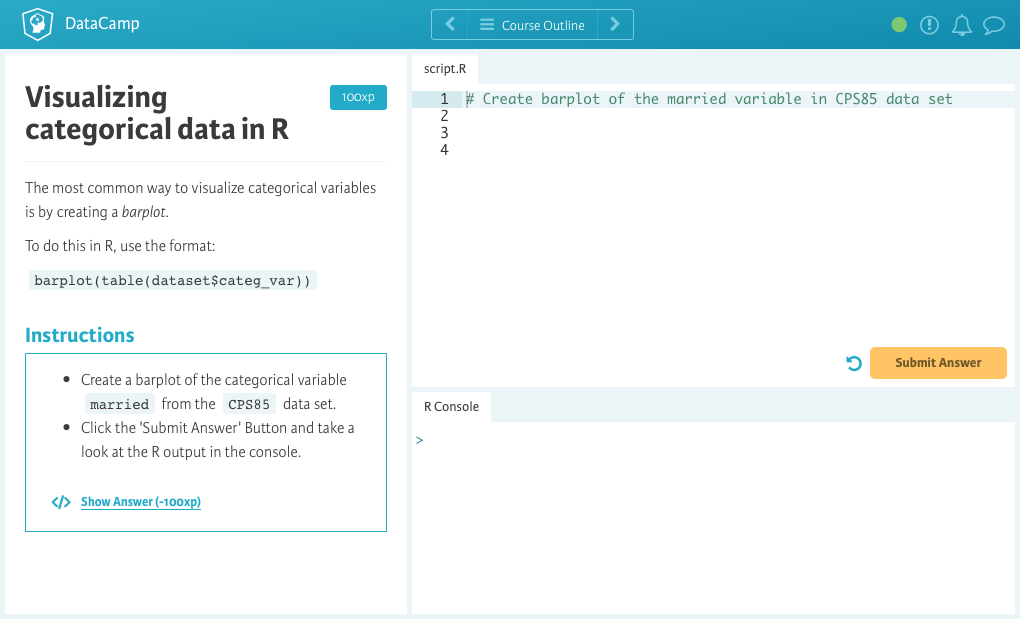
\includegraphics[scale = 0.19] {preview.jpg}
\end{figure}


Whenever a new exercise is added, DataCamp automatically produces the top line in the editor. The header specifies the type
of exercise (type), language (lang), available points (xp), skills learned (skills) and a 'key'. The key acts as a unique
identifier for that exercise, allowing you to modify the content without losing any student data. Currenly, DataCamp offers
eight different skills which are defined by numbers 1-8. The skills and their corresponding numbers can be found in the DataCamp
documentation \url{https://www.datacamp.com/teach/documentation#tab_gamification}. 
In the above exercise code, the 'type' is Normal, the language is R, the available points is 100 and the skills learned is 1 (which 
corresponds to *R Programming*. DataCamp assigns 100 points to normal coding exercises but this value can be modified depending on
difficulty level. After students have completed the exercise, they can check their personal profile to see how many points they earned.

In the 'assignment' portion of the exercise, instructors can add additional information about the assignment that will help
students understand and complete the instructions. The Instructions section will contain the actual task the student is
asked to execute. The 'pre-exercise code' sets up the workspace for the student; this section will contain code to import
data sets, install packages and any other operation that you want to be in the workspace but hidden from students. The 'sample
code' section contains code or notes that students view in the R script panel. Students also use the R script panel to write
the code that solves the tasks in the instructions. If students are not able to complete the task without help, they can click
on the 'Hint' button or eventually the 'solution'. When the student clicks the 'Submit Code' button, their answer passes through
the SCT code where the code is checked for errors.


The submission correctness testing code (or SCT) is the backbone for DataCamps' interactive nature. If a student submits an incorrect answer, they will 
receive immediate feedback on what they are doing wrong and the system will guide them to the right answer. Instructors can use the default feedback
that DataCamp automatically generates or write their own custom messages. The default feedback is meaningful and specific; most of the time custom 
messages are not necessary unless there is a common problem that student are struggling with in which more unique feedback is necessary. 
DataCamp provides a helpful R package called 'testwhat' which acts as a guide to writing and using SCTs (this can be accessed on DataCamp's GitHub 
repository: \url{https://github.com/datacamp/testwhat/wiki}. 
'testwhat' contains functions that can test different types of problems including loops, object definitions, printed output, functions, ect.
The submission correctness testing code compares the ideal answer (from the solution) to the students answer. Different
arguements can be added to the test functions to alter the testing process and automatic feedback. (**do I cite datacamp website here?**)

%add an example of a test_function sct.... maybe plot




The 'MultipleChoiceExercise', as you would expect, contains a question and a list of various answers. Instructors write the questions in the 'lesson'
portion of the exercise and offer solutions in the 'Insructions' section. Similar to the 'normal' coding exercises, the lesson, instructions, pre-exercise 
code and SCTs have to be specified but sample and solution code do not. DataCamp offers two types of multiple choice questions: simple and regular. 
The simple multiple choice exercises are used for questions that do not require the R console or any R output. Regular multiple choice exercises 
allow instructors to pre-program objects or plots that the student needs to access to answer the question. Both types of multiple choice exercises 
are straightforward to write can act as quick checks for understanding throughout the chapter.

%add example of regular multiple choice exercise --> use Quick check 2 from lab 8

Video exercises act as in instructional video addition to a DataCamp course; instructors can add short videos of them explaining concepts and with 
relevent slides that appear in the background. The DataCamp website \url{https://www.datacamp.com/teach/documentation#tab_code_exercises} provides 
more detail on the content of the various exercises. 


All DataCamp courses will have a course badge and most will use data sets and R packages. Information on how to add data sets and images
can be found in DataCamps 'Teach' documentation \url{https://www.datacamp.com/teach/documentation} under the 'Upload Assets' tab. However,
there is currently no information on DataCamp about integrating R packages. To use R packages in a course, you will need to create a new file
in the GitHub course repository named 'requirements.r'. The file should contain: $devtools::install_version$, package name and version for every
package you use in the DataCamp course. For example, following code will add the 'ggplot2' and 'mosaic' packages to the repository.

$$devtools::install_version("ggplot2", "2.2.0")$$
$$devtools::install_version("mosaic", "0.14.4")$$

In order for DataCamp to recognize this new file, you will need to add $$from: r-base-prod:27$$ to the course.yml file.

**How do I override the subscripts for devtools?**

%Check this out, Schubert said this \cite{Schubert13}.


%Check this out, Campbell said this \cite{Campbell02} regularly, but cite this in parentheses \citep{Campbell02}.


%Check this out, Chi said this \cite{Chi81}.

%Use this for final submission
%\bibliographystyle{ECA_jasa}
\bibliographystyle{Chicago}
\bibliography{TISE-DataCamp(Private Group)}
% before it was 'library' so I thought if I changed it to the new bib file it would work but it doesn't :(



\end{document}
